% GRNET-AWS resource request -- US-Foundation (NTUA Biomedical Engineering Laboratory)
% Build:  python docs/GRNET_AWS/budget.py   (regenerates generated/*.tex and figs/*.pdf)
%         cd docs/GRNET_AWS && latexmk -pdf proposal.tex
\documentclass[11pt,a4paper]{article}
\usepackage[T1]{fontenc}
\usepackage[utf8]{inputenc}
\usepackage{lmodern}
\usepackage{microtype}
\usepackage[a4paper,margin=2.1cm]{geometry}
\usepackage{graphicx}
\usepackage{booktabs}
\usepackage{tabularx}
\usepackage{array}
\usepackage{xcolor}
\usepackage{enumitem}
\usepackage{eurosym}
\usepackage[round,authoryear]{natbib}
\usepackage[font=small,labelfont=bf,skip=4pt]{caption}
\usepackage{subcaption}
\usepackage{float}
\usepackage{longtable}
\usepackage{needspace}
\usepackage{titlesec}
\usepackage[colorlinks=true,linkcolor=blue!45!black,citecolor=blue!45!black,urlcolor=blue!45!black]{hyperref}

\titleformat{\section}{\large\bfseries}{\thesection.}{0.5em}{}
\titlespacing*{\section}{0pt}{12pt}{5pt}
\setlist{nosep,leftmargin=1.3em}
\setlength{\parskip}{3pt}
\setlength{\parindent}{0pt}
\renewcommand{\arraystretch}{1.12}
\renewcommand{\EUR}[1]{\euro\,#1}
\newcommand{\para}[1]{\textbf{#1}\ }
\newcommand{\confirm}[1]{\textcolor{red!70!black}{[#1]}}
\newcommand{\CalcLink}{\confirm{AWS Pricing Calculator link -- create it from Appendix~A and paste it here}}

% generated by budget.py -- do not edit
\newcommand{\SlackPct}{25}
\newcommand{\PackingPct}{90}
\newcommand{\ContPct}{20}
\newcommand{\NodeUSDh}{27.44705}
\newcommand{\NodeUSDhShort}{27.45}
\newcommand{\GPUUSDh}{3.43}
\newcommand{\EUNodeUSDh}{34.29}
\newcommand{\EUPremiumPct}{24.9}
\newcommand{\EUExtraUSD}{4,189}
\newcommand{\PfiveUSDh}{6.88}
\newcommand{\PfourdUSDh}{21.96}
\newcommand{\PfourdGPUUSDh}{2.74}
\newcommand{\HBreakEven}{2.0}
\newcommand{\FX}{1.1355}
\newcommand{\FXdate}{2026-09-29}
\newcommand{\PriceDate}{2026-09-25}
\newcommand{\GPUhMeasured}{2,920}
\newcommand{\GPUhBudget}{3,649}
\newcommand{\GPUhPacked}{4,055}
\newcommand{\GPUhBilled}{4,896}
\newcommand{\NodeH}{612}
\newcommand{\NodeDays}{25.5}
\newcommand{\NodeHMonth}{102.0}
\newcommand{\NodeUSD}{16,798}
\newcommand{\ComputeUSD}{16,930}
\newcommand{\TotalUSD}{17,580}
\newcommand{\TotalEUR}{15,483}
\newcommand{\RequestEUR}{15,483}
\newcommand{\MonthlyUSD}{2,930}
\newcommand{\MonthlyEUR}{2,580}
\newcommand{\NodeSharePct}{96}
\newcommand{\NRuns}{396}
\newcommand{\OneGPUDays}{152}
\newcommand{\TwoGPUDays}{76}
\newcommand{\EpochTwoTwoFour}{0.82}
\newcommand{\EpochTwoTwoFourMin}{49}
\newcommand{\EpochFiveOneEight}{3.42}
\newcommand{\ImgsTwoTwoFour}{64.6}
\newcommand{\ImgsFiveOneEight}{15.5}
\newcommand{\ResRatio}{4.2}
\newcommand{\PaperRecipeH}{95.7}
\newcommand{\FullResH}{342}
\newcommand{\PtwoRunH}{8.8}
\newcommand{\PtwoRuns}{22}
\newcommand{\PtwoMaxH}{15.8}
\newcommand{\PtwoEpochs}{86}
\newcommand{\PtwoMinEpoch}{6.1}
\newcommand{\FullFTH}{19.6}
\newcommand{\FullFTMinEpoch}{13.1}
\newcommand{\ProbeH}{2.1}
\newcommand{\ProbeRuns}{14}
\newcommand{\OOFH}{1.9}
\newcommand{\TestFiveH}{0.67}
\newcommand{\SecPerImg}{0.99}
\newcommand{\RgSSL}{3.5}
\newcommand{\RgSSLhi}{3.4}
\newcommand{\RgPtwo}{2.5}
\newcommand{\RgProbe}{2.7}
\newcommand{\RbSSL}{0.38}
\newcommand{\RbPtwo}{0.56}
\newcommand{\ParamRatio}{3.7}
\newcommand{\TokenRatio}{5.3}
\newcommand{\BenchAgreePct}{4}
\newcommand{\LongestJob}{ViT-g: SSL bulk, 60 ep at 224 px}
\newcommand{\LongestJobH}{216}
\newcommand{\LongestJobDays}{9.0}
\newcommand{\GPUhWPZero}{19}
\newcommand{\USDWPZero}{87}
\newcommand{\EURWPZero}{77}
\newcommand{\GPUhWPOne}{501}
\newcommand{\USDWPOne}{2,307}
\newcommand{\EURWPOne}{2,032}
\newcommand{\GPUhWPTwo}{1,012}
\newcommand{\USDWPTwo}{4,657}
\newcommand{\EURWPTwo}{4,101}
\newcommand{\GPUhWPThree}{865}
\newcommand{\USDWPThree}{3,983}
\newcommand{\EURWPThree}{3,508}
\newcommand{\GPUhWPFour}{895}
\newcommand{\USDWPFour}{4,119}
\newcommand{\EURWPFour}{3,627}
\newcommand{\GPUhWPFive}{357}
\newcommand{\USDWPFive}{1,644}
\newcommand{\EURWPFive}{1,448}
\newcommand{\USDperAh}{4.60}
\newcommand{\CostPtwoRun}{50}
\newcommand{\CostProbe}{12}
\newcommand{\CostPaperSSL}{551}
\newcommand{\CostViTgSSL}{1,665}
\newcommand{\MVSNodeH}{288}
\newcommand{\MVSUSD}{8,688}
\newcommand{\MVSEUR}{7,651}
\newcommand{\MVSPct}{49}

\makeatletter
\newcommand{\tabinput}[1]{\@@input #1 }% primitive input: expandable, so \bottomrule may follow
\makeatother

\begin{document}

\begin{center}
{\LARGE\bfseries Detailed Project Document}\\[3pt]
{\large Request for Amazon Web Services resources through GRNET}
\end{center}

\begin{tabularx}{\textwidth}{@{}>{\bfseries}p{3.9cm}X@{}}
\toprule
Project name & US-Foundation: Scaling Self-Supervised Ultrasound Foundation Models for Generalizable Multi-Task Biometry \\
Research field & Biomedical Engineering -- Medical Image Analysis and Artificial Intelligence \\
Scientific supervisor & Prof.\ George K.\ Matsopoulos, Professor, School of Electrical and Computer Engineering, National Technical University of Athens (\texttt{gmatsopoulos@biomed.ntua.gr}) \\
Institution / laboratory & Biomedical Engineering Laboratory, School of Electrical and Computer Engineering, National Technical University of Athens (NTUA), Athens, Greece \\
Research team & Alexandros Barmperis (PhD candidate, technical lead; NTUA and Archimedes Research Unit, Athena Research Center; \texttt{amparmperis@biomed.ntua.gr}), Anna Panagiotakopoulou (NTUA), Vasileios E.\ Katsigiannis (NTUA) \\
Requested AWS services & Amazon EC2: one \texttt{p4de.24xlarge} (8$\times$ NVIDIA A100-SXM4-80GB) On-Demand, a \texttt{t3.large} control node and a 12-hour \texttt{p5.4xlarge} (H100) pilot; Amazon EBS (gp3); Amazon S3 (Standard); internet data transfer \\
AWS Region & US East (N.~Virginia), \texttt{us-east-1} -- the lowest A100-80GB price of all AWS Regions; fallback US West (Oregon), \texttt{us-west-2}, at the same price \\
Duration & 6 months (renewable), counted from the activation of the credits \\
Estimated cost & \$\TotalUSD{} = \EUR{\TotalEUR} at the ECB reference rate of \FXdate{} (1\,\euro{} = \FX{} US\$); \textbf{requested amount: \EUR{\RequestEUR}} \\
Cost estimate & \CalcLink \\
\bottomrule
\end{tabularx}

% ==========================================================================================
\section{Research project description}

\para{Summary.} Ultrasound is the most widely used imaging modality in pregnancy care and cardiology because it is safe, portable and inexpensive. Many clinical decisions rest on a few measurements taken on the image: the head and abdominal circumference and the femur length of a fetus, which track its growth; the angle of progression, which tracks labour; the size of the heart chambers and of the inferior vena cava. Each measurement is computed from a handful of anatomical \emph{landmarks} that a sonographer places by hand, which is slow, varies between operators, and is sensitive to the scanner used \citep{salomon2019isuog,ghi2018isuog,mitchell2019comprehensive}. This project develops \emph{one} artificial-intelligence model that places these landmarks automatically for nine different clinical tasks, and studies how to make it generalize across hospitals, scanners and tasks. The model starts from a general-purpose vision \emph{foundation model} (DINOv2, trained by Meta on 142 million natural images; \citealp{oquab2023dinov2}), adapts it to ultrasound with 191,170 unlabeled frames through self-supervised learning, which needs no manual labels, and then learns to place landmarks from 6,768 labeled images. The first version was built for the MICCAI~2026 Foundation Model Challenge for Ultrasound Biometry \citep{gu_biometry} and is described in our camera-ready challenge paper \citep{panagiotakopoulou2026fub}. The requested AWS credits fund the controlled, repeated experiments that are needed to turn this prototype into a reliable, openly released ultrasound landmark foundation model.

\para{Significance: impact and timeliness.} \emph{Clinically}, automated biometry shortens examinations and removes inter-observer variability, and a single model for prenatal, intrapartum and cardiac/vascular tasks is far simpler to validate and deploy than nine task-specific tools; multi-centre benchmarks show that site and scanner differences degrade single-task models \citep{divece2026multicentre,bai2026beyond}. \emph{Scientifically}, ultrasound foundation models are only now emerging \citep{jiao2024usfm,ambsdorf2025general,lin2025uusic}, and they target classification, segmentation or few-shot analysis; unified \emph{sparse landmark localization} across biometric domains is largely unexplored, and the new nine-task benchmark \citep{gu_biometry,deng2026baseline} makes it measurable for the first time. The work is \emph{timely} because our challenge entry exposed two questions that decide whether such models can be trusted and that can only be settled by large, controlled experiments: how self-supervised adaptation should be scheduled, and why gains measured internally did not transfer to the hidden test set.

\para{How the framework works (in brief).} The pipeline (Fig.~\ref{fig:method}) separates domain-level representation learning from task-specific localization. \emph{Phase~1} adapts the register variant of DINOv2-L/14 \citep{darcet2024registers} to unlabeled ultrasound by continued self-supervised pretraining that follows the DINOv2 recipe: CLS-token self-distillation \citep{caron2021dino}, masked patch-token prediction \citep{zhou2022ibot} and a KoLeo spread regularizer \citep{sablayrolles2018spreading}, with an exponential-moving-average (EMA) teacher, 2 global and 6 local crops, 65,536 prototypes and an effective batch of 256. Training runs mostly at a cheap 224-px resolution and ends with a short 518-px ``tail'' at the deployment resolution; the augmentations are ultrasound-specific (crops restricted to the imaging fan, gentle $\pm$10$^\circ$ rotations, masking restricted to tissue). \emph{Phase~2} feeds a 518$\times$518 letterboxed image through the adapted encoder, taps four depths (blocks 5, 11, 17, 23), and fuses them in an HRNet-style multi-resolution neck \citep{sun2019hrnet} with branches at 37$\times$37, 74$\times$74 and 148$\times$148 and GroupNorm throughout. Nine task-specific heads, selected by the task of each batch, output landmark heat-maps that a soft-argmax \citep{nibali2018numerical} turns into sub-pixel coordinates, mapped back to original-image pixels. The model is trained with a masked $L_1$ loss in original-pixel units, a task-balanced sampler and layer-wise learning-rate decay, and checkpoints are selected on a criterion aligned with the official challenge metric: 50\,\% landmark error plus 50\,\% clinical-measurement error, macro-averaged with equal weight per task.

\begin{figure}[t]
\centering
\begin{subfigure}{0.74\textwidth}\centering
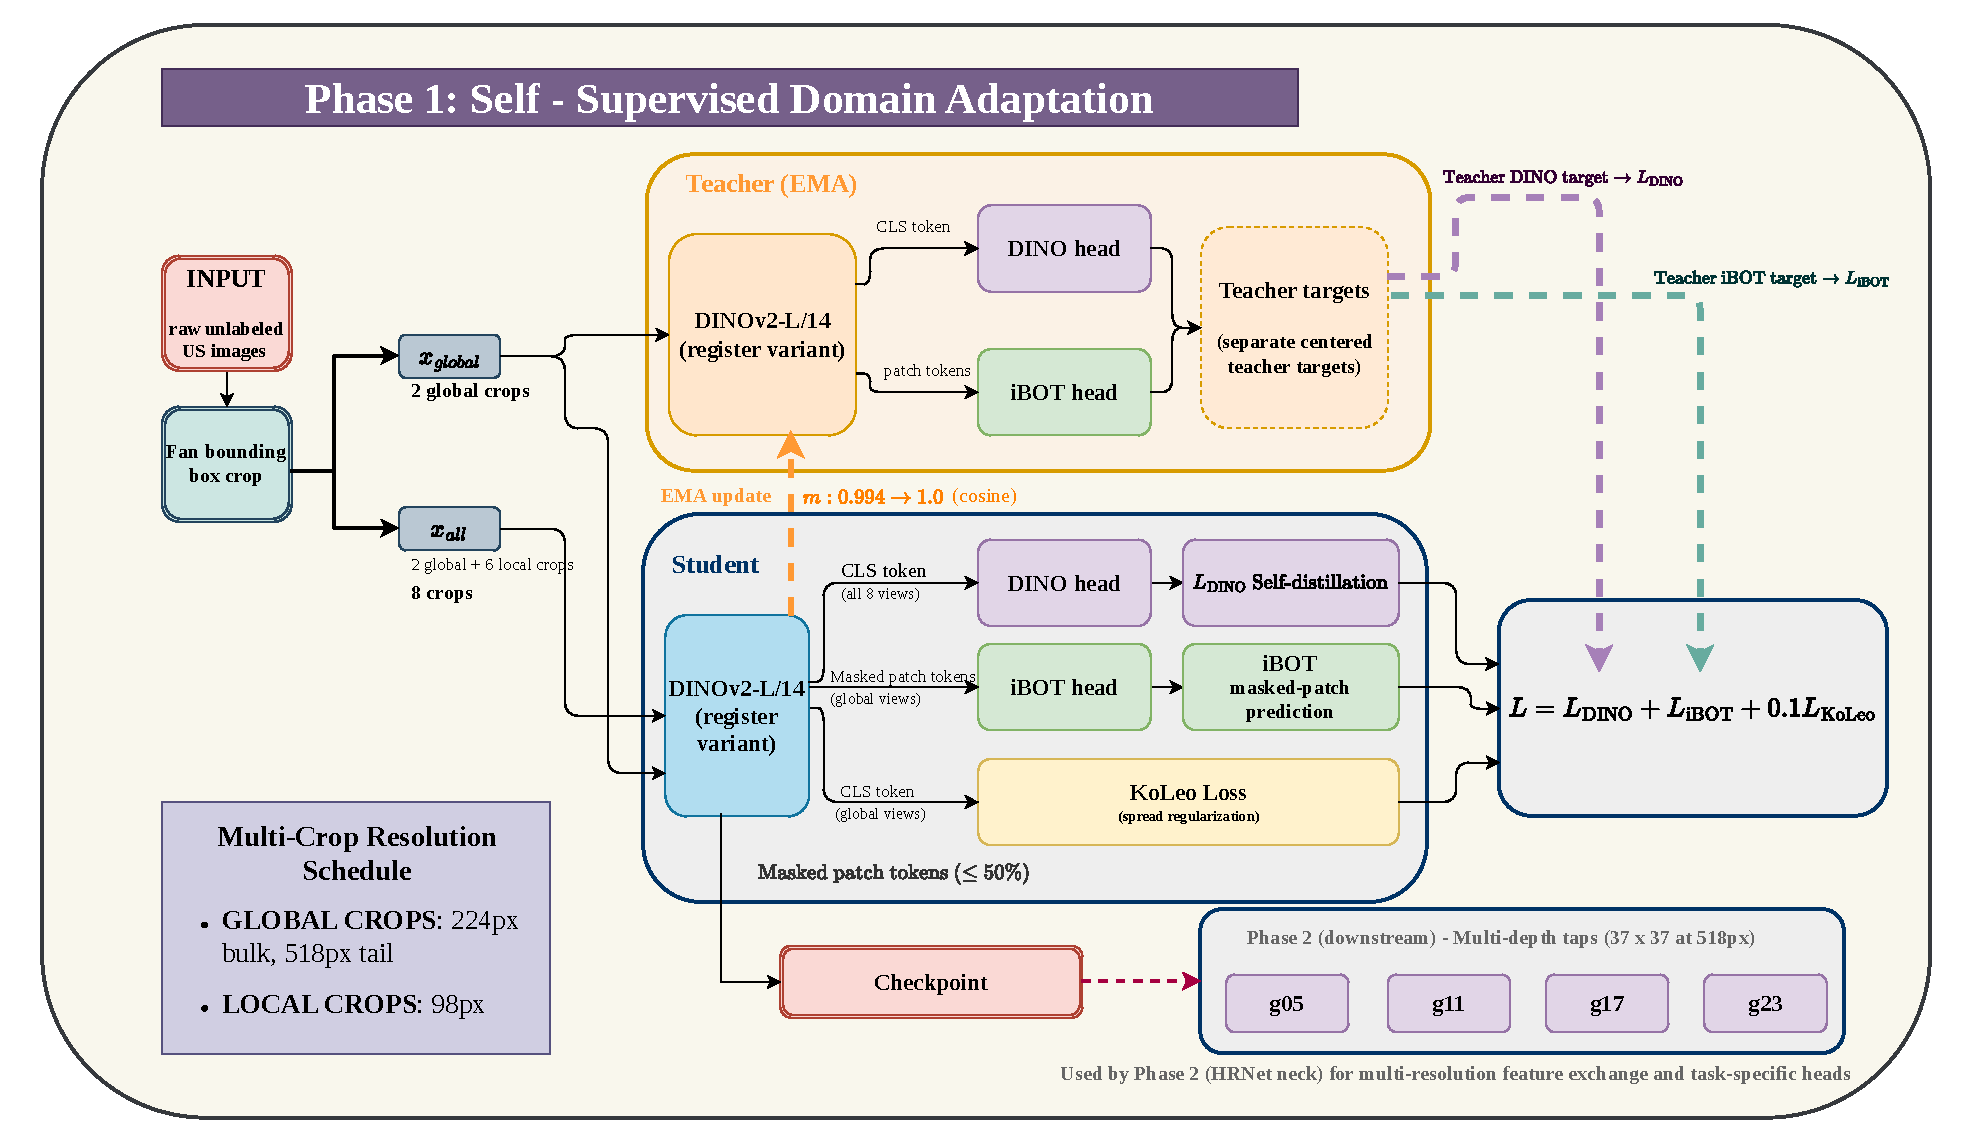
\includegraphics[width=\linewidth]{../MWM_54/figures/fig1_phase1_pipeline.pdf}
\caption{Phase~1: self-supervised domain adaptation of DINOv2-L/14 on 191,170 unlabeled frames.}
\end{subfigure}\\[4pt]
\begin{subfigure}{\textwidth}\centering
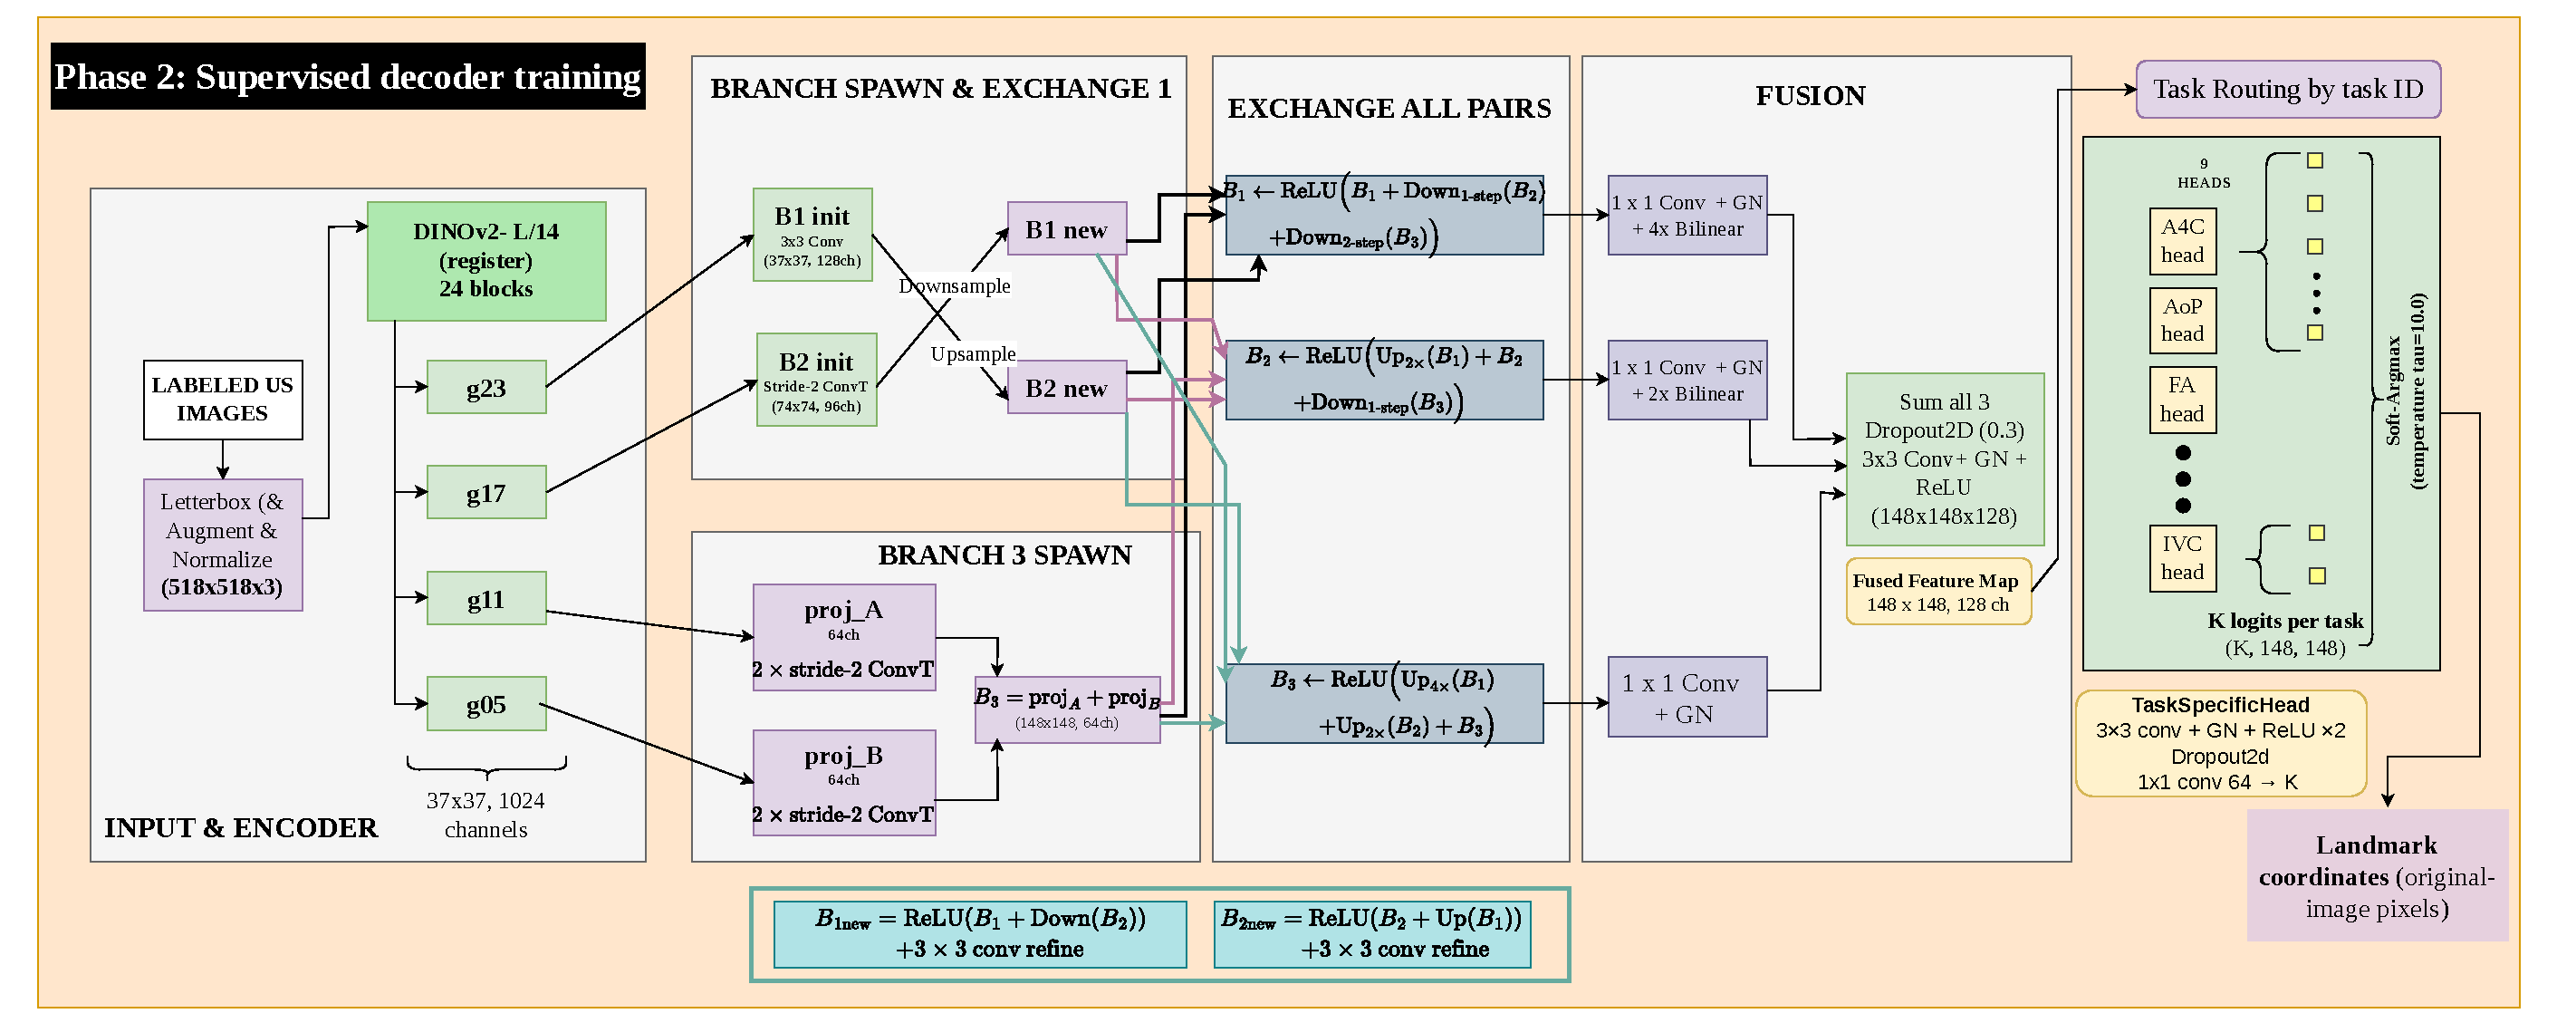
\includegraphics[width=\linewidth]{../MWM_54/figures/fig2_hrnet_neck.pdf}
\caption{Phase~2: multi-depth taps, HRNet-style neck, task routing to nine heads and soft-argmax decoding.}
\end{subfigure}
\caption{The two-phase pipeline \citep[figures reproduced from][]{panagiotakopoulou2026fub}.}
\label{fig:method}
\end{figure}

\para{What is already established.} On the official validation set (619 images, nine tasks) our single model reaches a mean radial error (MRE) of 26.34\,px and a measurement error (MAE) of 29.70; the best leaderboard entry reported 22.56\,px / 29.02. On the hidden test set the final submission obtained 30.66\,px / 36.78, and one task degraded sharply: the angle-of-progression MRE rose from 16.0\,px (validation) to 65.0\,px (test). Frozen-encoder probes (Fig.~\ref{fig:ssl}) show that ultrasound self-supervision is useful but \emph{non-monotonic}: 20 epochs at 224\,px lower the MRE from 31.27\,px (no adaptation) to 24.70\,px, whereas 100 epochs score worse than no adaptation on the selection criterion; a 4-epoch 518-px tail recovers the best score of all checkpoints (0.0747 vs.\ 0.0974 without the tail). Full-resolution training is not better at matched epochs and costs \ResRatio$\times$ more per epoch. Two further observations limit how far these conclusions can be trusted: (i) a five-fold comparison of decoders gave differences (0.0707\,$\pm$\,0.0089 vs.\ 0.0740\,$\pm$\,0.0068) smaller than the fold-to-fold spread, and (ii) our internal audit found that image-level folds leak cine loops, since in fold~0, 45\,\% of the A4C and 24\,\% of the PLAX validation frames come from a loop that also has frames in training. Leakage of this kind is a documented cause of over-optimistic medical-imaging results \citep{varoquaux2022failures,kapoor2023leakage}, and is a plausible reason why internal gains did not transfer to the hidden test.

\begin{figure}[t]
\centering
\begin{subfigure}{0.49\textwidth}\centering
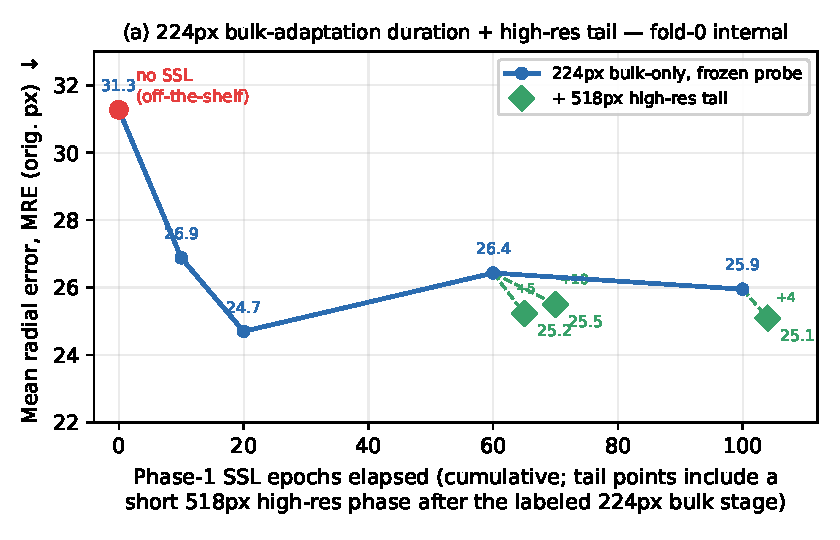
\includegraphics[width=\linewidth]{../MWM_54/figures/fig4a_ssl_duration_224.pdf}
\caption{224-px adaptation, with 518-px tails.}
\end{subfigure}\hfill
\begin{subfigure}{0.49\textwidth}\centering
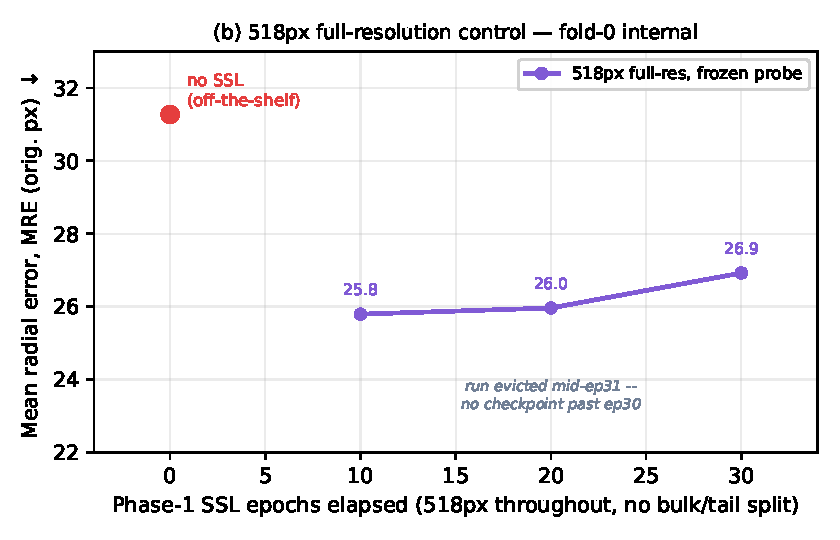
\includegraphics[width=\linewidth]{../MWM_54/figures/fig4b_ssl_duration_fullres.pdf}
\caption{518-px adaptation throughout (control).}
\end{subfigure}
\caption{Frozen-encoder probe MRE (original px) versus self-supervised adaptation length, fold~0, single seed \citep{panagiotakopoulou2026fub}. The non-monotonic curve is the central finding that WP2 must confirm over seeds and leakage-free folds.}
\label{fig:ssl}
\end{figure}

\para{Scientific questions.} The project is organized around four questions.
\begin{enumerate}[label=\textbf{(Q\arabic*)},leftmargin=2.6em]
\item \emph{Robust evaluation.} Which of the conclusions above survive a leakage-free, cine-loop-grouped five-fold cross-validation, and does the leakage-free internal score predict the hidden-test ranking?
\item \emph{Self-supervised schedule and data.} How long, at which resolution, and on how much unlabeled data should a general-purpose encoder be adapted to ultrasound? Is the non-monotonic duration curve reproducible over seeds, and where should the high-resolution tail start and how long should it last?
\item \emph{Capacity.} Does the benefit of in-domain self-supervision grow or shrink with encoder size, from ViT-B/14 (87\,M parameters) through ViT-L/14 (304\,M) to ViT-g/14 (1.14\,B) \citep{dosovitskiy2021image,zhai2022scaling}?
\item \emph{Phase-2 design.} Which decoder and training choices (multi-level fusion, fine-tuning depth from 0 to 24 blocks, measurement-aware and robust losses, task-sampling temperature) change the official metric by more than the fold-and-seed noise?
\end{enumerate}
The deliverable is an openly released ultrasound landmark foundation model (five-fold ensemble with test-time augmentation and ensemble-based uncertainty; \citealp{lakshminarayanan2017ensembles}), its code, and a leakage-free evaluation protocol for the nine-task benchmark.

\para{Why numerical experiments are the effective tool.} None of these questions can be answered analytically: the behaviour of a 304\,M--1.14\,B-parameter transformer adapted on 191,170 images can only be measured, by training many variants under identical conditions and repeating them over folds and seeds, because the fold-to-fold spread (13--15\,\%) is as large as the effects of interest \citep{bouthillier2021variance}. One self-supervised run of the published recipe took \PaperRecipeH{} A100-hours, a single fine-tuning run takes \PtwoRunH{} A100-hours on average, and the full plan comprises \NRuns{} GPU jobs (\GPUhMeasured{} A100-hours at measured rates). This is far beyond what our shared hardware can deliver in six months (Section~\ref{sec:why}).

% ==========================================================================================
\section{Work plan and management of the requested resources}

\para{Strategy.} All jobs are independent single-GPU runs (folds, seeds and configurations), so the campaign maps directly onto one \texttt{p4de.24xlarge} node with eight A100-80GB GPUs, the same GPU model on which every timing in this document was measured. The node is run in \emph{bursts}: it is started only when a queue of at least eight jobs is ready, runs eight jobs concurrently, and is stopped as soon as the queue drains, so that no GPU-hour is paid while idle. A small \texttt{t3.large} control node holds the job queue, synchronizes results and monitors spending. Datasets, checkpoints and logs live in Amazon S3, and each run writes an atomic \texttt{latest\_checkpoint} every epoch, so any interruption costs at most one epoch. The longest single job, the ViT-g self-supervised run (\LongestJobH{} budgeted hours, \LongestJobDays{} days), fixes the length of the largest burst; the other seven GPUs are filled with WP2--WP4 jobs during it.

\para{Work packages.} Budgeted A100-hours include the \SlackPct\,\% per-job slack of Section~\ref{sec:budget}.
\begin{itemize}
\item \textbf{WP0 -- Set-up, timing parity, H100 pilot (M1, \GPUhWPZero{} A100-h).} Account, quota (96 vCPUs of On-Demand P instances), S3 and EBS set-up; upload of the 20\,GB dataset and existing checkpoints; one SSL epoch at each resolution, one fine-tuning run and one probe, to confirm that AWS timings match Table~\ref{tab:unit} within $\pm$10\,\%; a 12-hour benchmark on one H100 (\texttt{p5.4xlarge}) to decide whether single-GPU H100 instances would be cheaper for the longest jobs.
\item \textbf{WP1 -- Leakage-free re-baselining, Q1 (M1--M2, \GPUhWPOne{} A100-h).} New cine-loop-grouped five-fold splits; six reference Phase-2 configurations $\times$ 5 folds; frozen probes of the 12 existing encoders $\times$ 5 folds; out-of-fold predictions for every ensemble, compared against our hidden-test results.
\item \textbf{WP2 -- SSL schedule, resolution and data, Q2 (M2--M4, \GPUhWPTwo{} A100-h).} Two new seeds of the 224-px trajectory with 518-px tails from epochs 20 and 60; a sweep of tail start (epochs 20/40/60) and length (2/5/10 epochs); continuation of the full-resolution control, which was evicted at epoch 30 on our shared node, to epoch 60; unlabeled-data scaling with 10/25/50\,\% subsets at matched compute; five-fold probes of all 22 new checkpoints and five-fold fine-tuning of the three best.
\item \textbf{WP3 -- Encoder capacity, Q3 (M3--M5, \GPUhWPThree{} A100-h).} The same protocol for ViT-B/14 and ViT-g/14 (60 bulk epochs, tails from epochs 20 and 60, five-fold probes, five-fold fine-tuning with and without adaptation); ViT-L results come from WP1--WP2.
\item \textbf{WP4 -- Phase-2 design and objectives, Q4 (M4--M5, \GPUhWPFour{} A100-h).} Fine-tuning depth of 8, 12 and 24 blocks; two alternative tap sets; measurement-aware, Wing and smooth-$L_1$ losses; sampler temperature and augmentation strength; two extra seeds of the best configuration, all over five leakage-free folds.
\item \textbf{WP5 -- Final ensembles, uncertainty and release (M5--M6, \GPUhWPFive{} A100-h).} Final ViT-L ensemble (5 folds $\times$ 3 seeds) and ViT-g ensemble (5 folds), all-data models, multi-scale/intensity test-time augmentation, ensemble-spread uncertainty, Docker image, public code and weights, final report.
\end{itemize}

\begin{figure}[H]
\centering
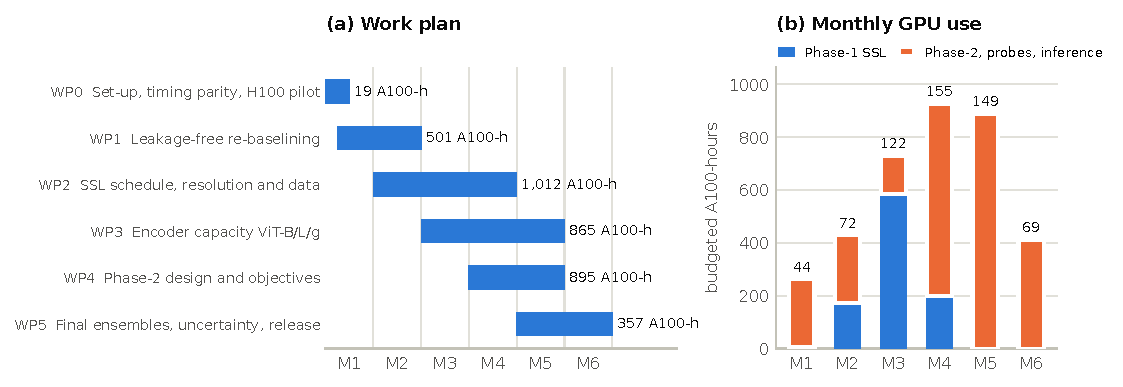
\includegraphics[width=\textwidth]{figs/fig_schedule.pdf}
\caption{(a) Six-month schedule with the budgeted A100-hours of each work package. (b) Monthly budgeted A100-hours split into self-supervised pretraining (Phase~1) and supervised runs, probes and inference (Phase~2); the label on each column is the \texttt{p4de.24xlarge} node-hours of that month, including packing and contingency.}
\label{fig:schedule}
\end{figure}

\begin{table}[H]
\centering\small
\caption{Monthly resource consumption. A100-hours are budgeted (with slack); node-hours and cost include packing and contingency, and the cost includes the storage, control-node and pilot lines of Table~\ref{tab:services}.}
\label{tab:months}
\begin{tabularx}{\textwidth}{@{}l>{\raggedright\arraybackslash}Xrrrrr@{}}
\toprule
Month & Main activities & SSL A100-h & Phase-2 A100-h & Node-h & USD & EUR \\
\midrule
\tabinput{generated/tab_months.tex}
\bottomrule
\end{tabularx}
\end{table}

% ==========================================================================================
\section{Numerical methods, algorithms, codes and libraries}

\para{Numerical methods and algorithms.} The numerical core is stochastic-gradient training of vision transformers \citep{dosovitskiy2021image} with mixed-precision (bfloat16) arithmetic, AdamW, cosine learning-rate, weight-decay and momentum schedules, gradient accumulation to an effective batch of 256, gradient clipping and EMA teachers. Phase~1 implements self-distillation with centred and sharpened teacher targets over 65,536 prototypes \citep{caron2021dino}, block-wise masked patch prediction \citep{zhou2022ibot} and the Kozachenko--Leonenko entropy estimator \citep{sablayrolles2018spreading}, as in DINOv2 \citep{oquab2023dinov2}. Phase~2 implements multi-resolution feature exchange \citep{sun2019hrnet}, differentiable soft-argmax coordinate regression with an optional DSNT regularizer \citep{nibali2018numerical}, masked $L_1$/Wing/smooth-$L_1$ losses re-weighted to original-image pixels, layer-wise learning-rate decay, and a task-homogeneous batch sampler with temperature-controlled task frequencies (every forward pass runs exactly one task head). Inference inverts the letterbox transform exactly and averages predictions over ensemble members and multi-scale/intensity views, with mean, median or hierarchical (per-member, then across-member) reduction.

\para{Evaluation protocol and statistics.} Every comparison uses five cine-loop-grouped folds; headline comparisons use three seeds \citep{bouthillier2021variance}. We report the official metric, landmark MRE in original pixels plus clinical-measurement error (angle in degrees for AoP, lengths in pixels elsewhere), macro-averaged over the nine tasks. Our scorer reproduces the official evaluation outputs exactly, and checkpoints are selected on this metric, never on the training loss. Differences are tested with paired bootstrap confidence intervals and Wilcoxon signed-rank tests over images, with Holm correction. Encoder quality is measured separately from fine-tuning with frozen-encoder probes, because self-supervised loss values are not comparable across recipes.

\para{Codes, packages and libraries.} All experiments run through our Python package \texttt{gubiometry} (single CLI: \texttt{make-splits}, \texttt{phase1}, \texttt{phase2}, \texttt{kfold}, \texttt{predict}, \texttt{evaluate}), driven by one YAML file per run with command-line overrides; every run stores its full configuration and the MD5 hash of its Phase-1 checkpoint, so any model can be rebuilt exactly. Dependencies: PyTorch 2.x with CUDA~12 and cuDNN, DINOv2 through \texttt{torch.hub} (Apache-2.0), NumPy, OpenCV, Albumentations, PyYAML, TensorBoard and matplotlib. A Docker image of the inference pipeline already exists; it produced our final hidden-test submission fully offline. Code: \url{https://github.com/abarmper/US-Foundation} \confirm{confirm the repository is public before sending}.

\para{How the methods enable the research.} One code path trains every configuration identically, so each difference can be attributed to the single factor varied (Q2--Q4). Loop-grouped folds and seeds make the differences statistically testable (Q1). Because encoder size, resolution, tail length, data fraction and fine-tuning depth are all configuration parameters, the whole plan is a grid of independent single-GPU jobs, which is exactly the workload an eight-GPU cloud node runs efficiently.

% ==========================================================================================
\section{Why AWS -- suitability and scaling evidence}
\label{sec:why}

\para{Current systems and their limits.} All results so far were produced on an 8$\times$ A100-SXM4-80GB cloud node provided by the NVIDIA Academic Hardware Grant Program (MedViLA) and shared by several researchers. In practice we could use one or two GPUs at a time: when this document was written, all eight GPUs were occupied by jobs of other projects (3D segmentation and image-synthesis studies of the laboratory and its collaborators). Long jobs are fragile on a shared node. The 518-px control run had to be restarted six times after external interruptions and was abandoned at epoch 30 of 100, which is why that comparison in our paper stops early. The grant is also time-limited \confirm{confirm the end date of the NVIDIA grant allocation}. At the budgeted \GPUhBudget{} A100-hours, the plan would occupy two dedicated GPUs for \TwoGPUDays{} days, and more than that on a contended node. This is incompatible with a six-month timeline.

\para{Why AWS, and which instance.} The \texttt{p4de.24xlarge} provides the \emph{same} GPU (A100-SXM4-80GB) on which all our timings were measured, so the unit costs of Table~\ref{tab:unit} transfer without extrapolation. It also has 96 vCPUs, 1,152\,GiB of memory and 8$\times$1\,TB local NVMe, enough for eight concurrent data-loading pipelines. The 80\,GB memory is required: our measurements (Table~\ref{tab:scaling}) show 60\,GB for ViT-L self-supervision at 518\,px, and ViT-g needs 58--62\,GB even with micro-batches reduced to 16 (224\,px) and 4 (518\,px); micro-batches of 32 and 8 do not fit in 80\,GB at all. The cheaper A100-40GB node (\texttt{p4d}, \$\PfourdGPUUSDh{} per GPU-hour) therefore cannot run the 518-px tail or any ViT-g job at our settings. A single-GPU H100 (\texttt{p5.4xlarge}, \$\PfiveUSDh/h) costs \HBreakEven$\times$ an A100 GPU-hour, so it only pays off for jobs that run at least \HBreakEven$\times$ faster; the WP0 pilot measures this instead of assuming it.

\para{Which Region.} Figure~\ref{fig:regions} compares the On-Demand price per GPU-hour of both A100 instances in every Region that offers them (AWS price list of \PriceDate). The A100-80GB node is cheapest in \texttt{us-east-1} and \texttt{us-west-2} (\$\NodeUSDh{} per hour, i.e.\ \$\GPUUSDh{} per GPU-hour). We choose \texttt{us-east-1} and keep \texttt{us-west-2} as a same-price fallback. The challenge data are de-identified research data and no personal data are processed. Should an EU Region be preferred, \texttt{eu-central-1} (Frankfurt) offers the same node at \$\EUNodeUSDh/h (+\EUPremiumPct\,\%), which would add about \$\EUExtraUSD{} to the estimate.

\begin{figure}[t]
\centering
\begin{minipage}{0.47\textwidth}
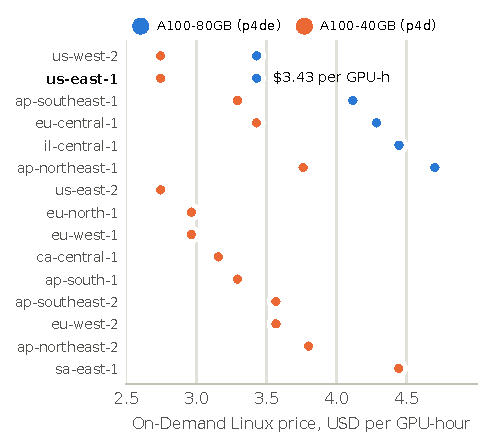
\includegraphics[width=\linewidth]{figs/fig_regions.pdf}
\end{minipage}\hfill
\begin{minipage}{0.5\textwidth}
\caption{On-Demand Linux price per GPU-hour of the A100-80GB (\texttt{p4de.24xlarge}) and A100-40GB (\texttt{p4d.24xlarge}) instances in every AWS Region that offers them, from the public AWS price list of \PriceDate. \texttt{us-east-1} (bold) and \texttt{us-west-2} share the lowest A100-80GB price, \$\GPUUSDh{} per GPU-hour; the A100-80GB instance is offered in six Regions only.}
\label{fig:regions}
\end{minipage}
\end{figure}

\para{Scaling evidence.} Table~\ref{tab:scaling} and Fig.~\ref{fig:scaling} report single-GPU throughput for the three encoder sizes, measured with our own training code on an idle A100-80GB. For ViT-L the benchmark agrees with the production logs within \BenchAgreePct\,\% for self-supervision; the fine-tuning log value is lower only because it includes the per-epoch validation pass. Cost grows \emph{sub-linearly} with model size: ViT-g has \ParamRatio$\times$ the parameters of ViT-L but costs \RgSSL$\times$ for self-supervision and \RgPtwo$\times$ for fine-tuning, because the frozen part of the encoder only runs forward. ViT-B costs \RbSSL$\times$ and \RbPtwo$\times$ of ViT-L. Resolution is the other lever: a 518-px global crop has \TokenRatio$\times$ the patch tokens of a 224-px crop, but an epoch costs only \ResRatio$\times$ more, and our curriculum spends 96\,\% of its epochs at the cheap resolution. Across jobs the scaling is linear: the jobs are independent, so eight GPUs complete the budgeted plan in \NodeH{} node-hours (\NodeDays{} days of node time), against \OneGPUDays{} days on one GPU.

\begin{table}[H]
\centering\small
\caption{Throughput in images/s on one A100-80GB (peak memory in brackets), same code path, bfloat16. Micro-batch 32 at 224\,px and 16 at 518\,px for SSL (``mb'' where ViT-g needed less), 64 for Phase~2. Production values are the ViT-L means from our training logs (Phase-2 values include validation). The last column is the time cost of ViT-g relative to ViT-L.}
\label{tab:scaling}
\begin{tabularx}{\textwidth}{@{}>{\raggedright\arraybackslash}Xccccc@{}}
\toprule
Workload & ViT-B/14 (87M) & ViT-L/14 (304M) & ViT-L, logs & ViT-g/14 (1.14B) & ViT-g cost \\
\midrule
\tabinput{generated/tab_scaling.tex}
\bottomrule
\end{tabularx}
\end{table}

\begin{figure}[t]
\centering
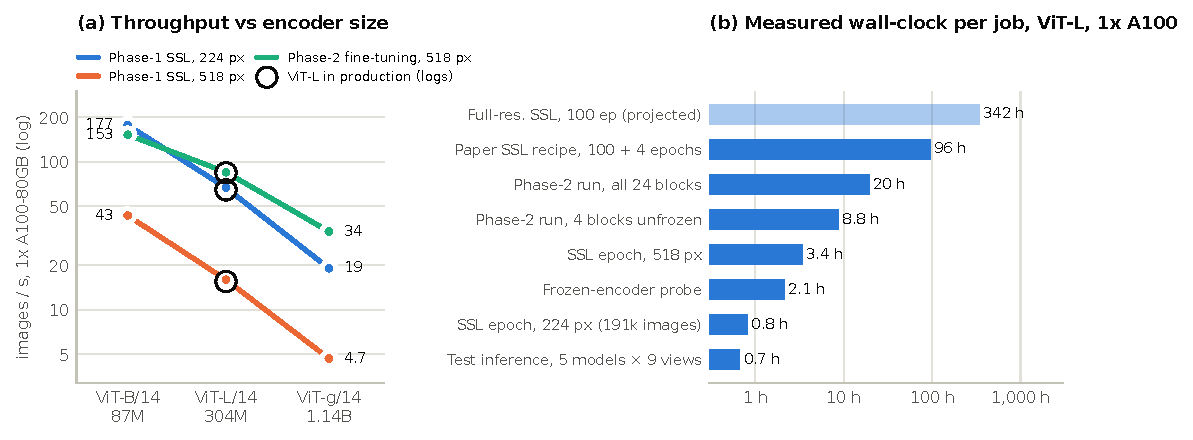
\includegraphics[width=\textwidth]{figs/fig_scaling.pdf}
\caption{Measured scaling on one A100-80GB. (a) Throughput versus encoder size for self-supervised pretraining (224 and 518\,px) and Phase-2 fine-tuning (log--log); black rings mark the ViT-L throughput of our production runs. (b) Measured wall-clock of each job type for ViT-L (log scale; the full-resolution run is projected from its measured epochs because it was never allowed to finish).}
\label{fig:scaling}
\end{figure}

\needspace{5\baselineskip}
\para{How the AWS credits will help.}
\begin{itemize}
\item \emph{They buy exactly the compute the plan needs:} \NodeH{} node-hours of 8$\times$ A100-80GB, i.e.\ \GPUhBilled{} A100-hours, at \$\USDperAh{} per budgeted A100-hour including packing and contingency. That is \$\CostPtwoRun{} per fine-tuning run, \$\CostProbe{} per probe and \$\CostPaperSSL{} per full self-supervised recipe, so every item in Table~\ref{tab:wp} has a known price.
\item \emph{Dedicated GPUs, no evictions:} eight GPUs per burst shorten the programme from months of shared-node time to \NodeDays{} days of node time, and uninterrupted multi-day jobs (the \LongestJobDays-day ViT-g run) become possible for the first time.
\item \emph{New science:} the capacity study of WP3 (ViT-B and ViT-g, \$\USDWPThree) and the leakage-free, multi-seed protocol of WP1--WP2 (\$\USDWPOne{} + \$\USDWPTwo) cannot be run on our current allocation.
\item \emph{Reproducibility and accountability:} S3 keeps every checkpoint, configuration and log; each resource is tagged with its work package, so the spend per work package can be reported to GRNET.
\end{itemize}

% ==========================================================================================
\section{Experience using cloud and HPC resources}

The team trains and serves all its models on GPU cloud instances. On the current 8$\times$A100 NVIDIA cloud node we manage our own environments, multi-GPU job chains, checkpoint/resume, and the Codabench Docker image that ran our final submission fully offline. We have also provisioned rented GPU instances (RunPod), including building the CUDA/PyTorch toolchain, and our laboratory uses a Slurm-managed GPU cluster for other projects. We have been allocated and operated compute by GRNET before, through its educational AWS programme, on which we provisioned and ran GPU compute on EC2 instances, so we are familiar with GRNET's allocation process and with EC2, EBS and S3. The workload needs no MPI and no inter-node communication: jobs are arrays of single-GPU runs, launched from YAML configurations and made robust by atomic per-epoch checkpoints with automatic resume, a scheme we already rely on.

% ==========================================================================================
\section{Justification of the requested budget}
\label{sec:budget}

\para{From measured timings to credits.} Every unit cost in Table~\ref{tab:unit} is measured from our A100-SXM4-80GB training logs (for example, 100 epochs of 224-px self-supervision took 82.1\,h), and every job of Table~\ref{tab:wp} is expressed in those units; ViT-B and ViT-g jobs are scaled by the measured ratios of Table~\ref{tab:scaling}. The work plan totals \GPUhMeasured{} A100-hours at measured rates. Slack is then added in three explicit steps (Table~\ref{tab:waterfall}). (1) \SlackPct\,\% on \emph{every} job covers differences in CPU and data loading on AWS (12 vCPUs per GPU instead of 32 on our node), early-stopping variability (runs last 45--150 epochs; we budget the mean), and checkpoint I/O. (2) Division by \PackingPct\,\% packing efficiency pays for GPU slots that stay idle while the node is up, since \texttt{p4de} bills all eight GPUs. (3) A \ContPct\,\% contingency covers failed or repeated runs, debugging, extra seeds where a comparison turns out to be borderline, and changes in AWS prices or in the exchange rate during the allocation. The result, \NodeH{} node-hours, is rounded up to whole hours per month so that the AWS Pricing Calculator reproduces it exactly.

\begin{table}[H]
\centering\small
\caption{Unit costs on one A100-80GB: measured from our training logs, then budgeted with +\SlackPct\,\% slack; the cost column uses the effective \$\USDperAh{} per budgeted A100-hour (packing and contingency included).}
\label{tab:unit}
\begin{tabularx}{\textwidth}{@{}>{\raggedright\arraybackslash}Xrrrl@{}}
\toprule
Job (ViT-L unless stated) & Measured h & Budgeted h & Cost & Source \\
\midrule
\tabinput{generated/tab_unit.tex}
\bottomrule
\end{tabularx}
\end{table}

{\small
\setlength{\LTpre}{2pt}
\begin{longtable}{@{}p{0.635\textwidth}rrrr@{}}
\caption{Work plan in A100-hours: number of jobs, measured hours per job, total at measured rates, and budgeted total with +\SlackPct\,\% slack. ViT-B/ViT-g jobs are scaled by the measured ratios of Table~\ref{tab:scaling}.}\label{tab:wp}\\
\toprule
Job & \# & h/job & Measured & Budgeted \\
\midrule
\endfirsthead
\toprule
Job & \# & h/job & Measured & Budgeted \\
\midrule
\endhead
\tabinput{generated/tab_wp.tex}
\midrule
\textbf{Total} & \textbf{\NRuns} & & \textbf{\GPUhMeasured} & \textbf{\GPUhBudget} \\
\bottomrule
\end{longtable}
}

\begin{table}[H]
\centering\small
\caption{From measured A100-hours to billed \texttt{p4de.24xlarge} node-hours.}
\label{tab:waterfall}
\begin{tabular}{@{}lrr@{}}
\toprule
Step & A100-hours & Node-hours \\
\midrule
\tabinput{generated/tab_waterfall.tex}
\bottomrule
\end{tabular}
\end{table}

\begin{table}[H]
\centering\footnotesize
\caption{Estimated cost by AWS service in \texttt{us-east-1} for the six-month allocation (AWS price list of \PriceDate; On-Demand, taxes excluded). Euro amounts use the ECB reference rate of \FXdate{}, 1\,\euro{} = \FX{} US\$. These lines are the entries of the AWS Pricing Calculator estimate (Appendix~\ref{app:calc}).}
\label{tab:services}
\setlength{\tabcolsep}{4pt}
\begin{tabularx}{\textwidth}{@{}l>{\raggedright\arraybackslash}Xrrrr@{}}
\toprule
Service & Configuration & Quantity & Unit price & USD & EUR \\
\midrule
\tabinput{generated/tab_services.tex}
\bottomrule
\end{tabularx}
\end{table}

\para{Requested amount.} The estimate is \$\TotalUSD{}, i.e.\ \EUR{\TotalEUR} at \FX{} US\$/\euro{}, and we request exactly this amount, \textbf{\EUR{\RequestEUR}}, for six months (\$\MonthlyUSD{} or \EUR{\MonthlyEUR} per month on average). The GPU node accounts for \NodeSharePct\,\% of it, and its hours are fully itemized in Table~\ref{tab:wp}. Storage is deliberately modest: a 1\,TB gp3 volume for the working set, the node's local NVMe as scratch, and S3 for about 1\,TB of datasets and retained checkpoints. We keep only the selected checkpoint of each finished run (1.2\,GB for ViT-L).

\para{Minimum viable subset.} If only part of the amount can be granted, WP0--WP2 plus the ViT-L part of WP5 (\MVSNodeH{} node-hours, \$\MVSUSD{} $\approx$ \EUR{\MVSEUR}, \MVSPct\,\% of the request) still answer Q1 and Q2 and deliver the released ViT-L model; the capacity study (Q3) and the Phase-2 design study (Q4) would then be dropped.

\para{Cost control.} Spending is monitored daily in AWS Cost Explorer, and AWS Budgets alerts fire at 50\,\%, 80\,\% and 100\,\% of each month's plan (Table~\ref{tab:months}). The node runs only while its queue is full and is stopped by the control node when it drains. S3 lifecycle rules delete intermediate checkpoints after evaluation. Where Spot capacity of the same instance is available at a lower price, short probe and inference jobs use it; any saving extends the contingency, not the scope.

% ==========================================================================================
\section{Data management, dissemination and acknowledgement}

The challenge data are de-identified images released for research; they are kept in a private, encrypted S3 bucket (server-side encryption, TLS in transit) accessible only to the project's IAM users, are never redistributed, and are deleted from AWS at the end of the allocation. Code, trained weights (within the Apache-2.0 terms of DINOv2) and the leakage-free fold definitions will be released openly with the resulting journal publication. As required by the programme, all publications that use these resources will state that \emph{``the resources were granted with the support of GRNET''}, and their citation records will be sent to \texttt{helpdesk@aws.grnet.gr}.

% ==========================================================================================
\small
\bibliographystyle{plainnat}
\bibliography{references}
\normalsize

\appendix
\section{AWS Pricing Calculator entries}
\label{app:calc}
The estimate is reproduced at \url{https://calculator.aws/} by adding the services below in \texttt{us-east-1} (On-Demand, Linux, shared tenancy) with the listed \emph{monthly} quantities; the calculator's monthly total times six months equals the estimate of Table~\ref{tab:services} and the requested amount.

\begin{table}[H]
\centering\small
\begin{tabularx}{\textwidth}{@{}ll>{\raggedright\arraybackslash}Xr@{}}
\toprule
Service & Region & Configuration (per month) & USD / month \\
\midrule
\tabinput{generated/tab_calculator.tex}
\bottomrule
\end{tabularx}
\end{table}

\section{Provenance of the numbers}
All figures and tables are generated by \path{docs/GRNET_AWS/budget.py} from three inputs in \path{docs/GRNET_AWS/data/}:
\begin{itemize}
\item \path{measured_timings.json}, parsed from the time-stamped epoch lines of our training logs by \path{tools/extract_timings.py} (\ImgsTwoTwoFour{} and \ImgsFiveOneEight{} images/s for SSL at 224 and 518\,px, \PtwoRuns{} fine-tuning runs, \ProbeRuns{} probes);
\item \path{bench_results.jsonl}, the ViT-B/L/g micro-benchmarks of \path{tools/bench_scaling.py}, which replicates the production training step;
\item \path{aws_prices.json}, fetched from the public AWS price list and the ECB reference rate by \path{tools/fetch_aws_prices.py}.
\end{itemize}
Re-running the three scripts before submission refreshes every number in this document.

\end{document}
